\documentclass[a4j,12pt,]{jarticle}
 \usepackage{float}
 \usepackage{siunitx} %%SI単位系用
 \usepackage{amssymb, amsmath}
 \usepackage{ascmac,here,txfonts}
 \usepackage{hyperref}
 \usepackage{listings}
 \usepackage{pxjahyper}
 \usepackage[dvipdfmx]{graphicx}
 \usepackage{amssymb, amsmath}
  \usepackage{listings}
  \usepackage[dvipdfmx]{color}
 
 \lstset{
   language={Python},
   basicstyle={\ttfamily},
   identifierstyle={\small},
   commentstyle={\small\itshape},
   keywordstyle={\small\bfseries},
   ndkeywordstyle={\small},
   stringstyle={\small\ttfamily},
   frame={single},
   breaklines=true,
   columns=[l]{fullflexible},
   numbers=left,
   xrightmargin=0zw,
   xleftmargin=3zw,
   numberstyle={\scriptsize},
   stepnumber=1,
   numbersep=1zw,
   lineskip=-0.5ex,
 }
\begin{document}

{\noindent\small 第18回報告書 \hfill\today}
\begin{center}
  {\Large 133.71.201.197のElasticSearchサーバーのデータの移行について}
\end{center}
\begin{flushright}
  祖父江匠真 \\
\end{flushright}

\section{概要}
今回は, 133.71.201.197のElasticSearchサーバーにあるpcs\_recyclekanという名前のインデックス以外のインデックスについて調査を行い, 133.71.106.141のElasticSearchサーバーにデータ移行を行った.

\section{133.71.201.197のElasticSearchサーバーにあるインデックスについて}
図 \ref{p1}に133.71.201.197のElasticSearchサーバーにあるインデックスの一覧を示す.

\begin{figure}[H]
  \begin{center}
    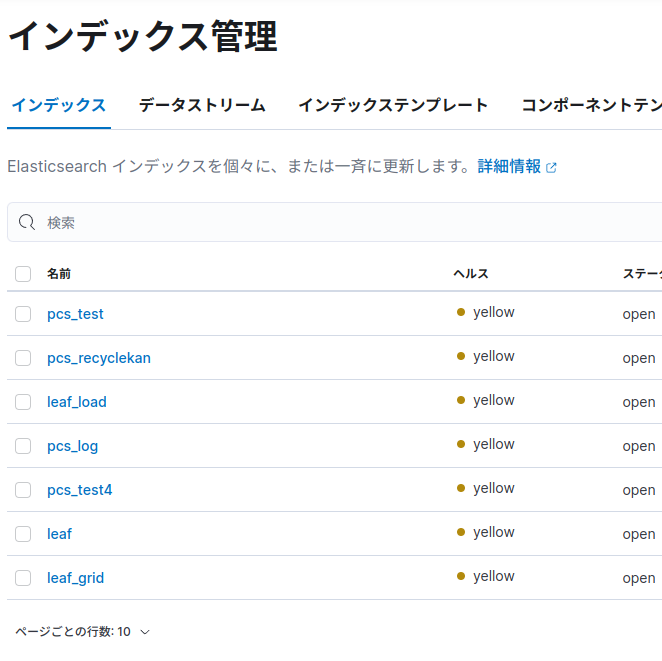
\includegraphics[width=160mm]{indexes.png}
    \caption{133.71.201.197のElasticSearchサーバーにあるインデックスの一覧}
    \label{p1}
  \end{center}
\end{figure}

これらのインデックスが保存しているデータについて説明する.

\begin{itemize}
  \item pcs\_test
  \begin{itemize}
    \item 恵村君がプログラムの検証目的で使用しているインデックス
  \end{itemize}
  \item pcs\_recyclekan
  \begin{itemize}
    \item リサイクル館の太陽光発電に関するデータを保存しているインデックス
  \end{itemize}
  \item leaf\_load
  \begin{itemize}
    \item leafのデータが保存されているインデックス
  \end{itemize}
  \item pcs\_log
  \begin{itemize}
    \item リサイクル館の太陽光発電に関するデータをElasticSearchにインサートするPythonプログラムのログ情報を保存しているインデックス
  \end{itemize}
  \item pcs\_test4
  \begin{itemize}
    \item 恵村君がプログラムの検証目的で使用しているインデックス
  \end{itemize}
  \item leaf
  \begin{itemize}
    \item leafのデータが保存されているインデックス
  \end{itemize}
  \item leaf\_grid
  \begin{itemize}
    \item leafのデータが保存されているインデックス
  \end{itemize}
\end{itemize}

pcs\_testインデックスとpcs\_test4インデックスに関しては, 検証用途で使用しているものであるため, 今回の移行対象からは除外し, pcs\_log, leaf, leaf\_load, leaf\_gridインデックスのみを移行対象とした.

\section{データ移行手順について}

データ移行手順について, まず移行元のElasticSearchサーバーのデータをローカルマシンにエクスポートして, 移行先のElasticSearchサーバーにデータをインサートした.

\subsection{データのエクスポート}
移行元のElasticSearchサーバーのデータのローカルマシンへのエクスポートには, elasticdump \cite{1}ライブラリを使用してJSON形式でエクスポートした.その際, pcs\_log, leaf, leaf\_load, leaf\_gridという名前のインデックスのデータをエクスポートした.

\subsection{データのインポート}
ダンプしたJSONファイルを作成したPythonプログラムで読み込んで, Pythonのelasticsearchライブラリを用いて移行先のElasticSearchサーバーにインサートした.

移行先のElasticSearchサーバーにおけるインデックス名については, 133.71.201.197のElasticSearchサーバーと同名のインデックスに保存した.

\section{データ移行が正常に行えたか確認}
図 \ref{p2}に移行元のElasticSearchサーバーのleafという文字列を含むインデックスのドキュメント数をカウントしたものを, 図 \ref{p3}に移行先のElasticSearchサーバーのleafという文字列を含むインデックスのドキュメント数をカウントしたものを示す.

図 \ref{p2}と図 \ref{p3}より, ドキュメント数が一致していることからデータ移行が正常に行えたと判断できる.

\begin{figure}[H]
  \begin{center}
    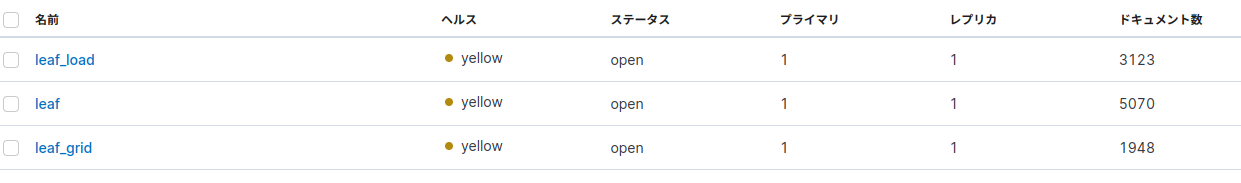
\includegraphics[width=160mm]{197leaf.png}
    \caption{133.71.201.197のElasticSearchサーバーのleafという文字列を含むインデックスのドキュメントのカウント結果}
    \label{p2}
  \end{center}
\end{figure}

\begin{figure}[H]
  \begin{center}
    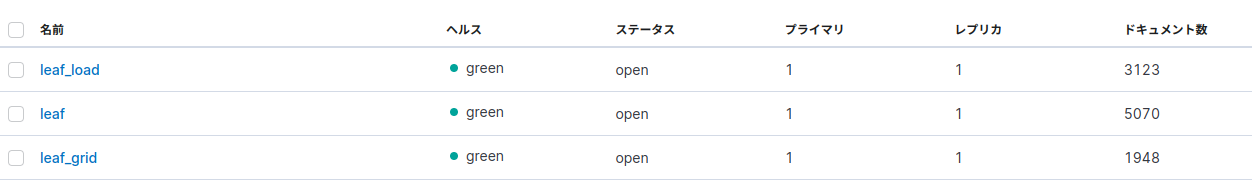
\includegraphics[width=160mm]{141leaf.png}
    \caption{133.71.106.141のElasticSearchサーバーのleafという文字列を含むインデックスのドキュメントのカウント結果}
    \label{p3}
  \end{center}
\end{figure}

次に, 図 \ref{p4}に移行元のElasticSearchサーバーのpcs\_logインデックスのドキュメント数をカウントしたものを, 図 \ref{p5}に移行先のElasticSearchサーバーのpcs\_logインデックスのドキュメント数をカウントしたものを示す.

図 \ref{p4}と図 \ref{p5}より, ドキュメント数が一致していることからデータ移行が正常に行えたと判断できる.

\begin{figure}[H]
  \begin{center}
    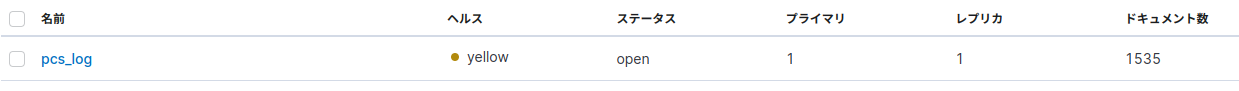
\includegraphics[width=160mm]{197pcs.png}
    \caption{133.71.201.197のElasticSearchサーバーのpcs\_logインデックスのドキュメントのカウント結果}
    \label{p4}
  \end{center}
\end{figure}

\begin{figure}[H]
  \begin{center}
    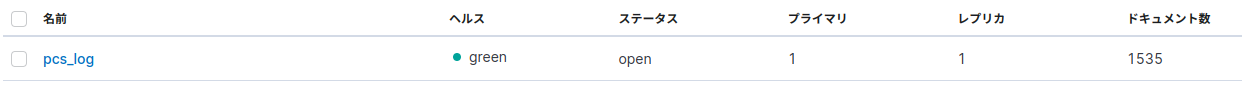
\includegraphics[width=160mm]{141pcs.png}
    \caption{133.71.106.141のElasticSearchサーバーのpcs\_logインデックスのドキュメントのカウント結果}
    \label{p5}
  \end{center}
\end{figure}

\section{まとめ}
今回は, 133.71.201.197のElasticSearchサーバーにあるpcs\_log, leaf, leaf\_load, leaf\_gridインデックスを133.71.106.141のElasticSearchサーバーにデータ移行して, 各インデックスのドキュメント数を比較することでデータ移行が正常に行えたことを報告した.

% pcs\_logインデックスは, 継続して133.71.201.197のElasticSearchサーバーにデータがインサートされているので, 恵村君が133.71.106.141のElasticSearchサーバーのpcs\_logインデックスにデータをインサートするようシステムの対応を行った時点で, 追加のデータ移行を行う必要がある.

次回は, 以前CO\textsubscript{2}データを移行した際にElasticSearchのBulk APIを使用してデータ移行を行ったことが原因で, ラズベリーパイ上で実行しているCO\textsubscript{2}データのインサート用のプログラムから移行先のElasticSearchサーバーのインデックスにインサートが出来なくなった問題について, 以前データ移行を行ったpcs\_recyclekanインデックスについてもBulk APIを使用しており, 将来同じ問題が発生する可能性があるため, 解決方法を調査する.

\begin{thebibliography}{5}
  \bibitem{1}Ferron H, ”ElasticDump”, https://github.com/elasticsearch-dump/elasticsearch-dump, 参照 June 19,2023.
\end{thebibliography}

\end{document}

